\documentclass[a4paper,10pt,twocolumn]{article}
\usepackage[utf8]{inputenc}
\usepackage{graphicx}
\usepackage[center]{caption}
\usepackage[english]{babel}
% \usepackage[top=3cm, bottom=3cm, left=2cm, right=2cm]{geometry}

%---------------------------------------------
% Font packages
%---------------------------------------------
\usepackage{lmodern}
% \usepackage{concmath}
% \usepackage{cmbright}
% \usepackage{kpfonts}
% \usepackage[adobe-utopia]{mathdesign}
% \usepackage{fouriernc}
\usepackage[T1]{fontenc}

%---------------------------------------------
% Math environment packages & command
%---------------------------------------------
\usepackage{amsmath}
\usepackage{amssymb}
\usepackage{array}
% \usepackage{mathrsfs}
\usepackage{array}
% \def\sgn{\mathop{\rm sgn}\nolimits} 
% \usepackage{bbm}


%---------------------------------------------
% item option
%---------------------------------------------
\renewcommand{\labelitemi}{-}


%---------------------------------------------
%HEADER & FOOTER
%---------------------------------------------
\usepackage{fancyhdr}
\pagestyle{fancy}

\renewcommand{\headrulewidth}{.15pt}
\fancyhead[C]{{\textsc{Classical Loop-Shaping}}} 
\fancyhead[L]{Page \thepage \ of \pageref{LastPage}}
\fancyhead[R]{EL2520}

\renewcommand{\footrulewidth}{.15pt}
\fancyfoot[C]{\thepage} 
% \fancyfoot[L]{truc}
\fancyfoot[R]{EE -- Automatic Control}

\usepackage{lastpage}

%---------------------------------------------
% two column option
%---------------------------------------------
\setlength{\columnsep}{1cm}

%---------------------------------------------
% Table of content
%---------------------------------------------
\usepackage[colorlinks,linkcolor=black, citecolor=black]{hyperref}

%---------------------------------------------
% Opening
%---------------------------------------------
\title{Computer Exercice:\\ \textsc{Classical Loop-Shaping}}
\author{Jean-Alix \textsc{David}, Kilian \textsc{Demeulemeester} \\ \texttt{\{jadavid,kiliande\}@kth.se}}

%---------------------------------------------
% Numerotation Handling
%---------------------------------------------
\setcounter{section}{3}
\usepackage[explicit]{titlesec}
% \titleformat{<command>}[<shape>]{<format>}{<label>}{<sep>}{<before>}[<after>]
\titleformat{\subsubsection}[hang]{\normalfont\normalsize\bfseries}%
    {}{4pt}%
    {#1 \arabic{section}.\arabic{subsection}.\arabic{subsubsection}}


%---------------------------------------------
% Dummy text
%---------------------------------------------
\usepackage{lipsum}

%---------------------------------------------
% Quote
%---------------------------------------------
\usepackage[babel=true]{csquotes}
    
\begin{document}

\setlength\parindent{0em}

 \maketitle

\tableofcontents

\begin{abstract}
 \begin{bfseries}
\emph{Abstract} -- 
Bla bla...
\end{bfseries}

\end{abstract}

\section{Exercises}

\subsection{Basics}

We consider a system which can be modeled by the transfer function:

$$ G(s) = \frac{3(-s+1)}{(5s+1)(10s+1)} $$

\subsubsection{Exercise}

We want to design a lead-lag controller which eliminates the static control error for a step response in the reference signal.

The controller transfer function is the following:

$$ F(s) = K \frac{\tau_D s + 1}{\beta \tau_D s + 1} \frac{\tau_I s + 1}{\tau_I s + \gamma}$$

We want to fulfill the following criteria:
\begin{itemize}
 \item Phase margin of $30^{\circ}$ at the cross-over frequency $\omega_c = 0.4$ rad/s.
 \item No static control error for a step response 
\end{itemize}

\subsubsection{Exercise} 

For the exercice above, the most important differences between the minimum phase and non-minimum phase case are:

\subsubsection{Exercise}

Using the method depicted in Exercice \ref{exo411} with $\tau_I = 1$s places the integral action too close to the cross-over frequency: The lag-action and the lead-action of the controller are overlapping.

Therefore, we increase the value of $\tau_I$ to $\tau_I = 10$s.

The resulting controller fulfill all the criteria. (see Figure \ref{figbode413} and \ref{figstep413}).

The lead lag controller with a phase-margin of $50^{\circ}$ has the following caracteristics:
\begin{center}
\begin{tabular}{|c|c|}
    \hline
    Bandwith ($-3dB$) & $[0,0.99]$(rad/s)\\
    \hline
    Resonance peak $M_T$ & $2.06$dB at $0.56$(rad/s)\\
    \hline
    Rise time $t_r$ & $2.22$ s\\
    \hline
    Overshoot $D$\% & $15.7$\%\\
    \hline
\end{tabular}
\end{center}

\begin{figure}[h!t]
   \includegraphics[width=\columnwidth]{fig/bode413.eps}
    \caption{Bode diagram of the system's functions \\ Phase-margin: $50^{\circ}$} 
    \label{figbode413}
\end{figure}

\begin{figure}[h!t]
   \includegraphics[width=\columnwidth]{fig/step413.eps}
    \caption{Step response of the system with and without the controller \\ Phase-margin: $50^{\circ}$}
    \label{figstep413}
\end{figure}






% \subsection{Disturbance attenuation}
% \subsubsection{Exercise} 


Figure \ref{min_glover_fig} shows the reaction of the minimum phase system. 

Figure \ref{nonmin_glover_fig} shows the reaction of the non-minimum phase system. 

See Table \ref{analysis_glover} for the analysis of the results. 

\begin{figure}[h!t]
        \centering
        \begin{subfigure}[b]{\columnwidth}
                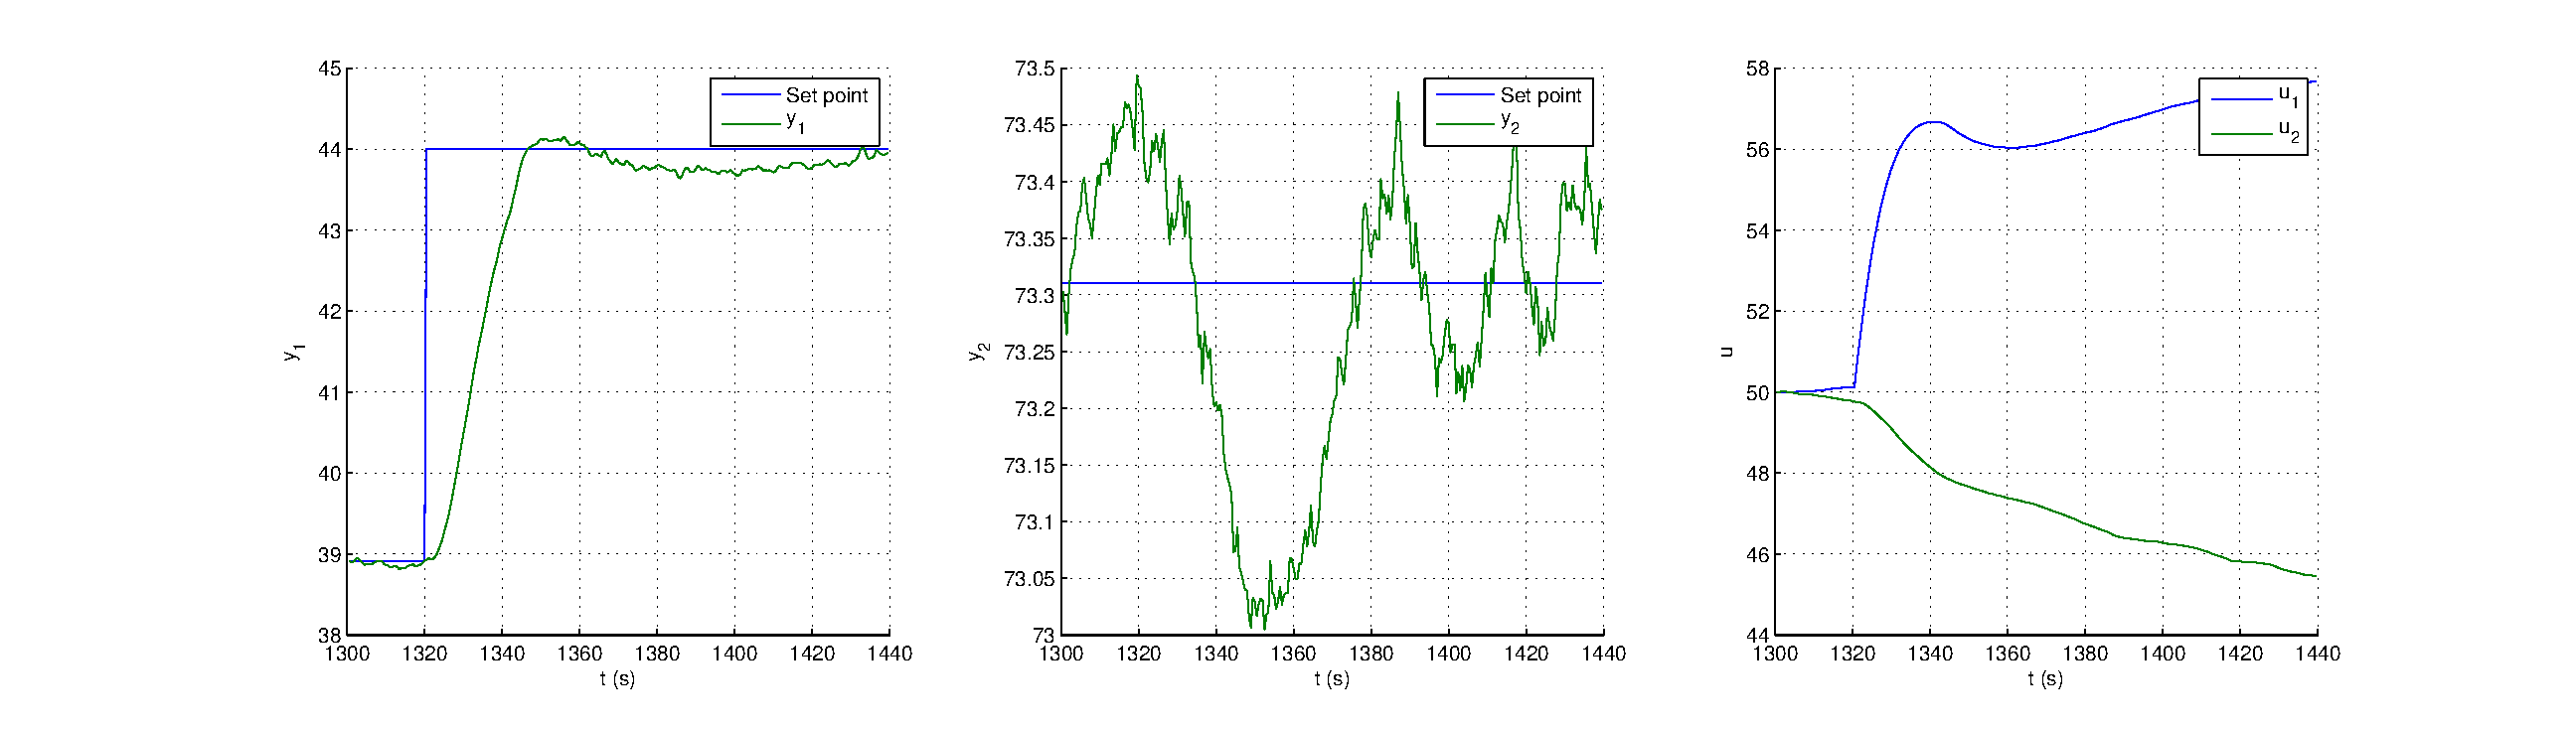
\includegraphics[width=\columnwidth]{fig/min_glover_step.eps}
                \caption{Step response}
        \end{subfigure}
        \begin{subfigure}[b]{\columnwidth}
                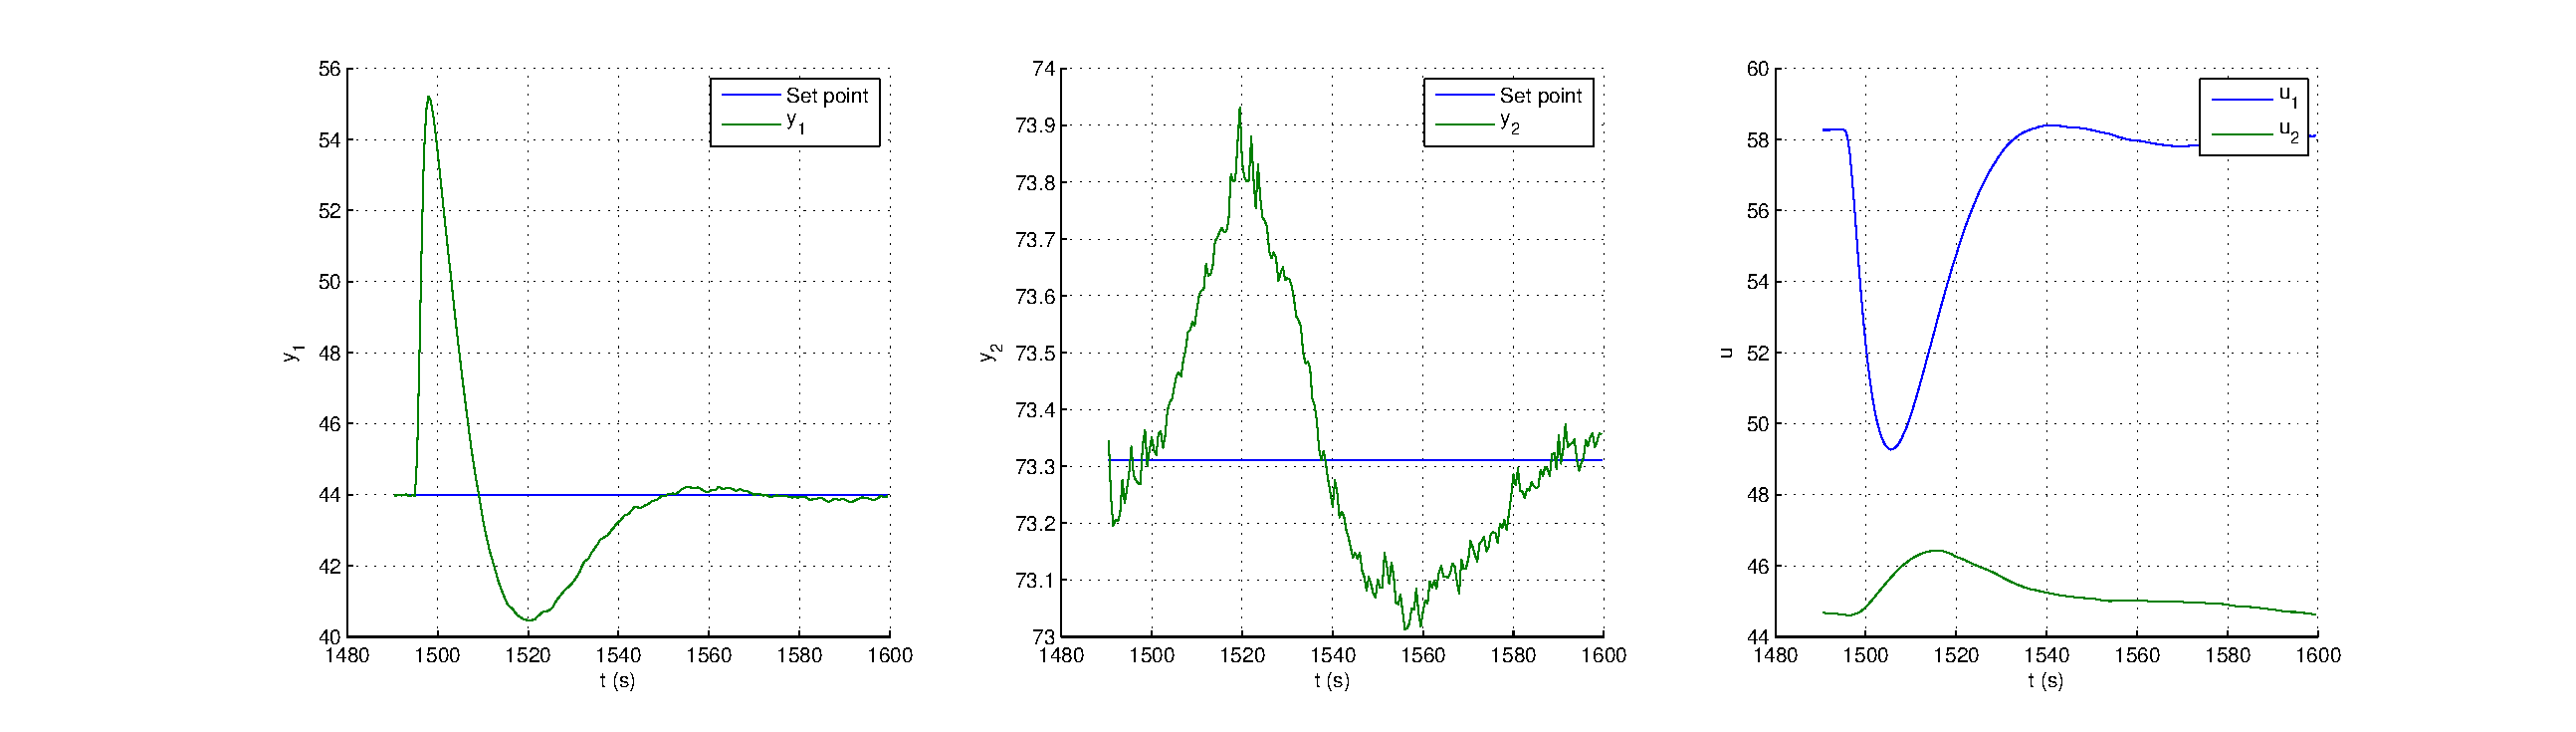
\includegraphics[width=\columnwidth]{fig/min_glover_gob.eps}
                \caption{Cup of water response}
        \end{subfigure}
        \begin{subfigure}[b]{\columnwidth}
                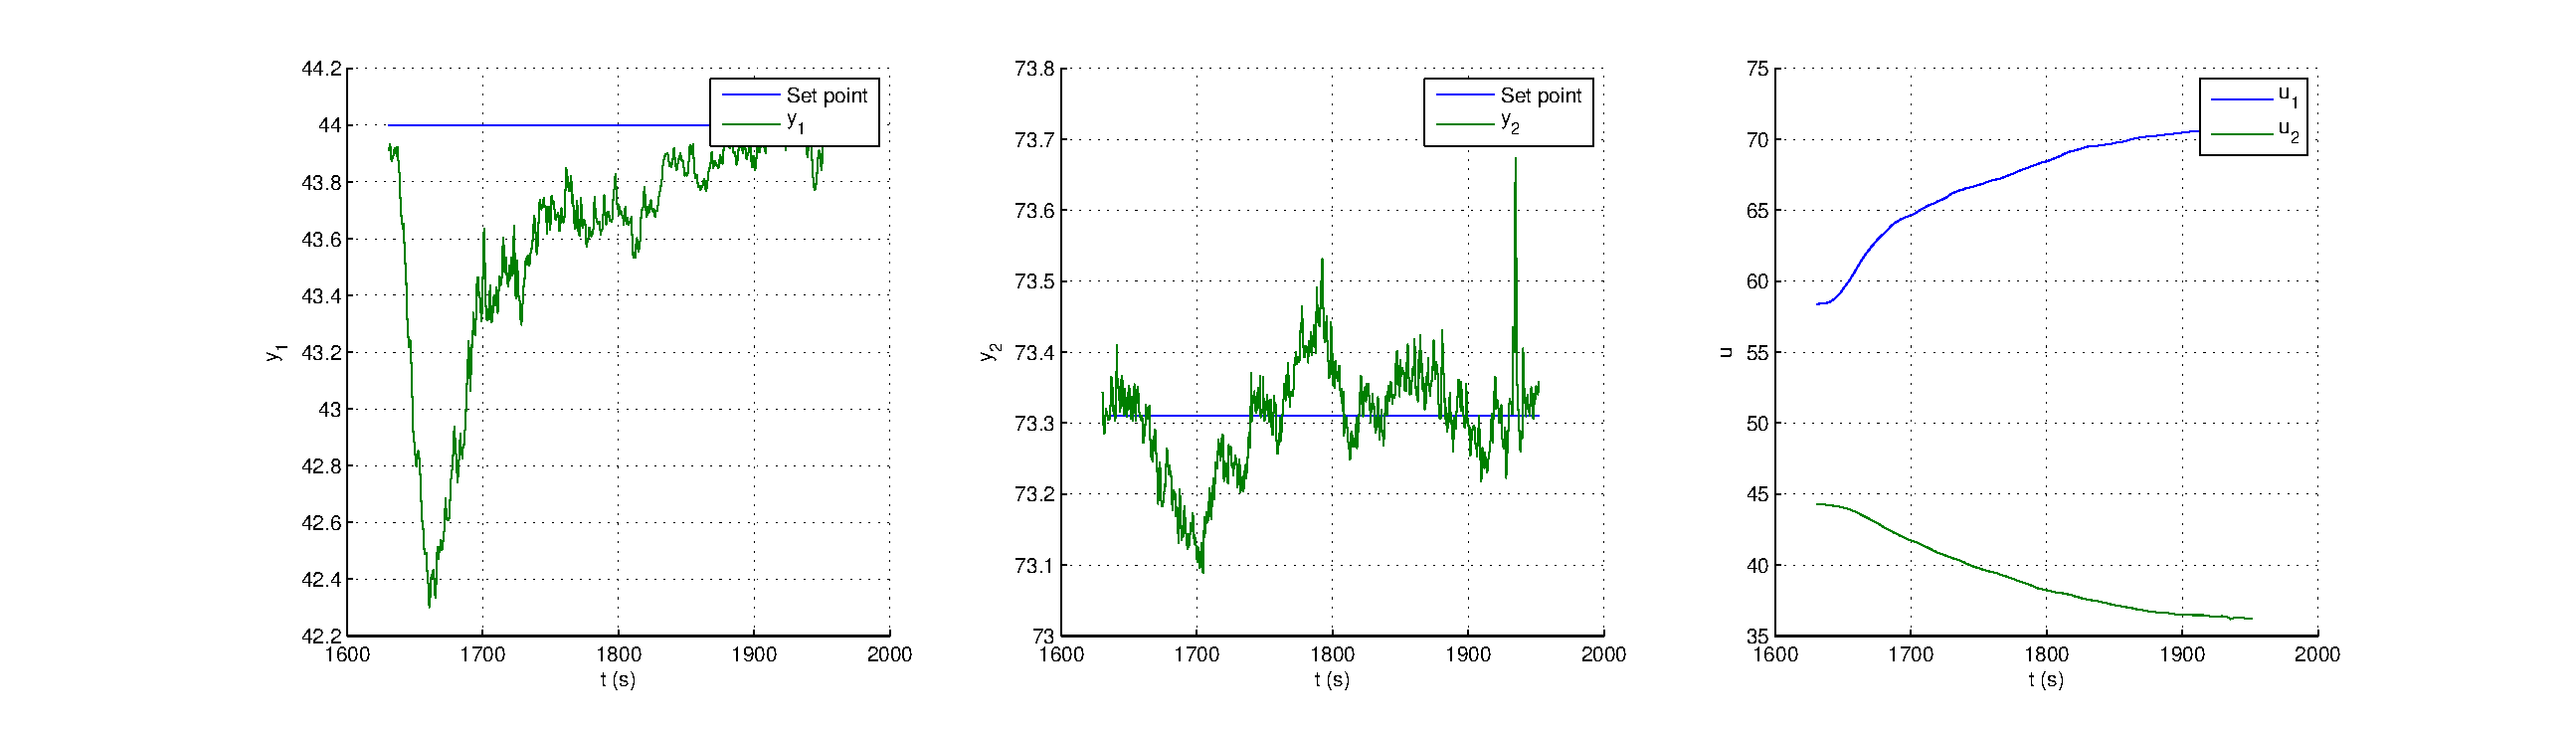
\includegraphics[width=\columnwidth]{fig/min_glover_fui.eps}
                \caption{Extra outlet response}
        \end{subfigure}
        \caption{Minimum phase system reactions \\ Glover-MacFarlane controller}
        \label{min_glover_fig}
\end{figure}

\begin{figure}[h!t]
        \centering
        \begin{subfigure}[b]{\columnwidth}
                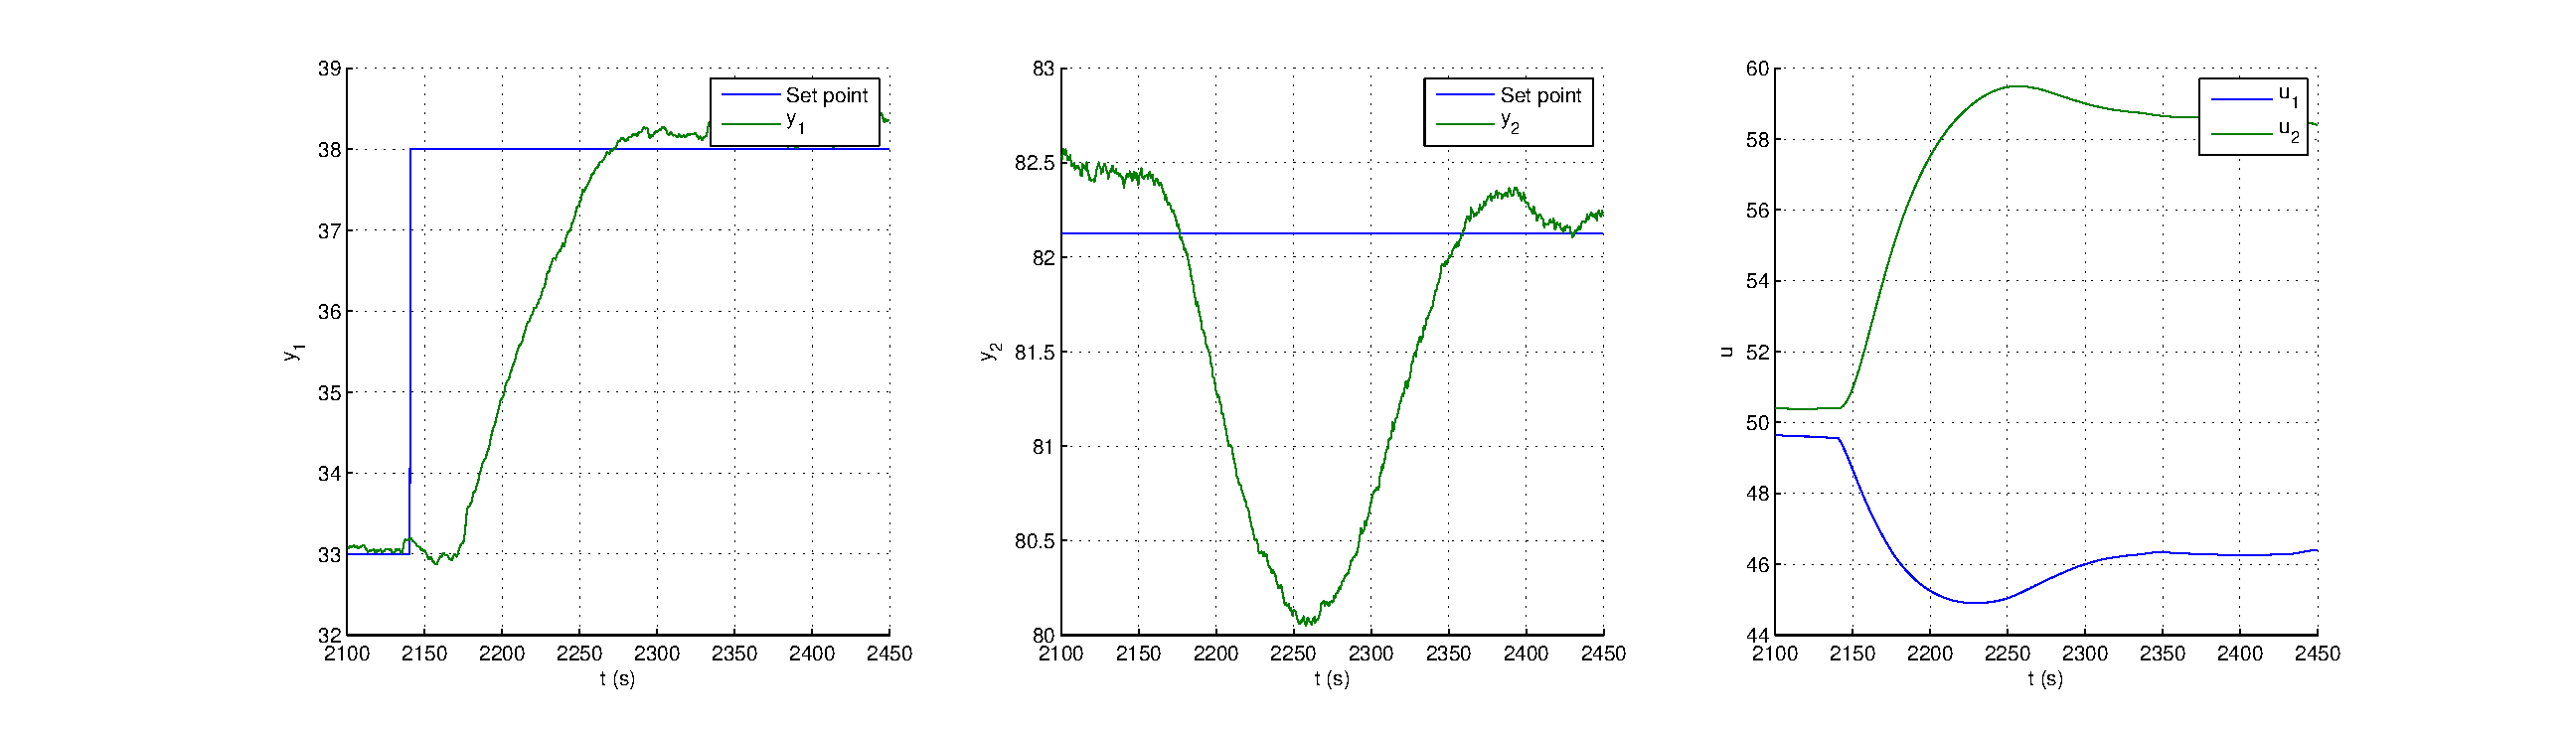
\includegraphics[width=\columnwidth]{fig/nonmin_glover_step.eps}
                \caption{Step response}
        \end{subfigure}
        \begin{subfigure}[b]{\columnwidth}
                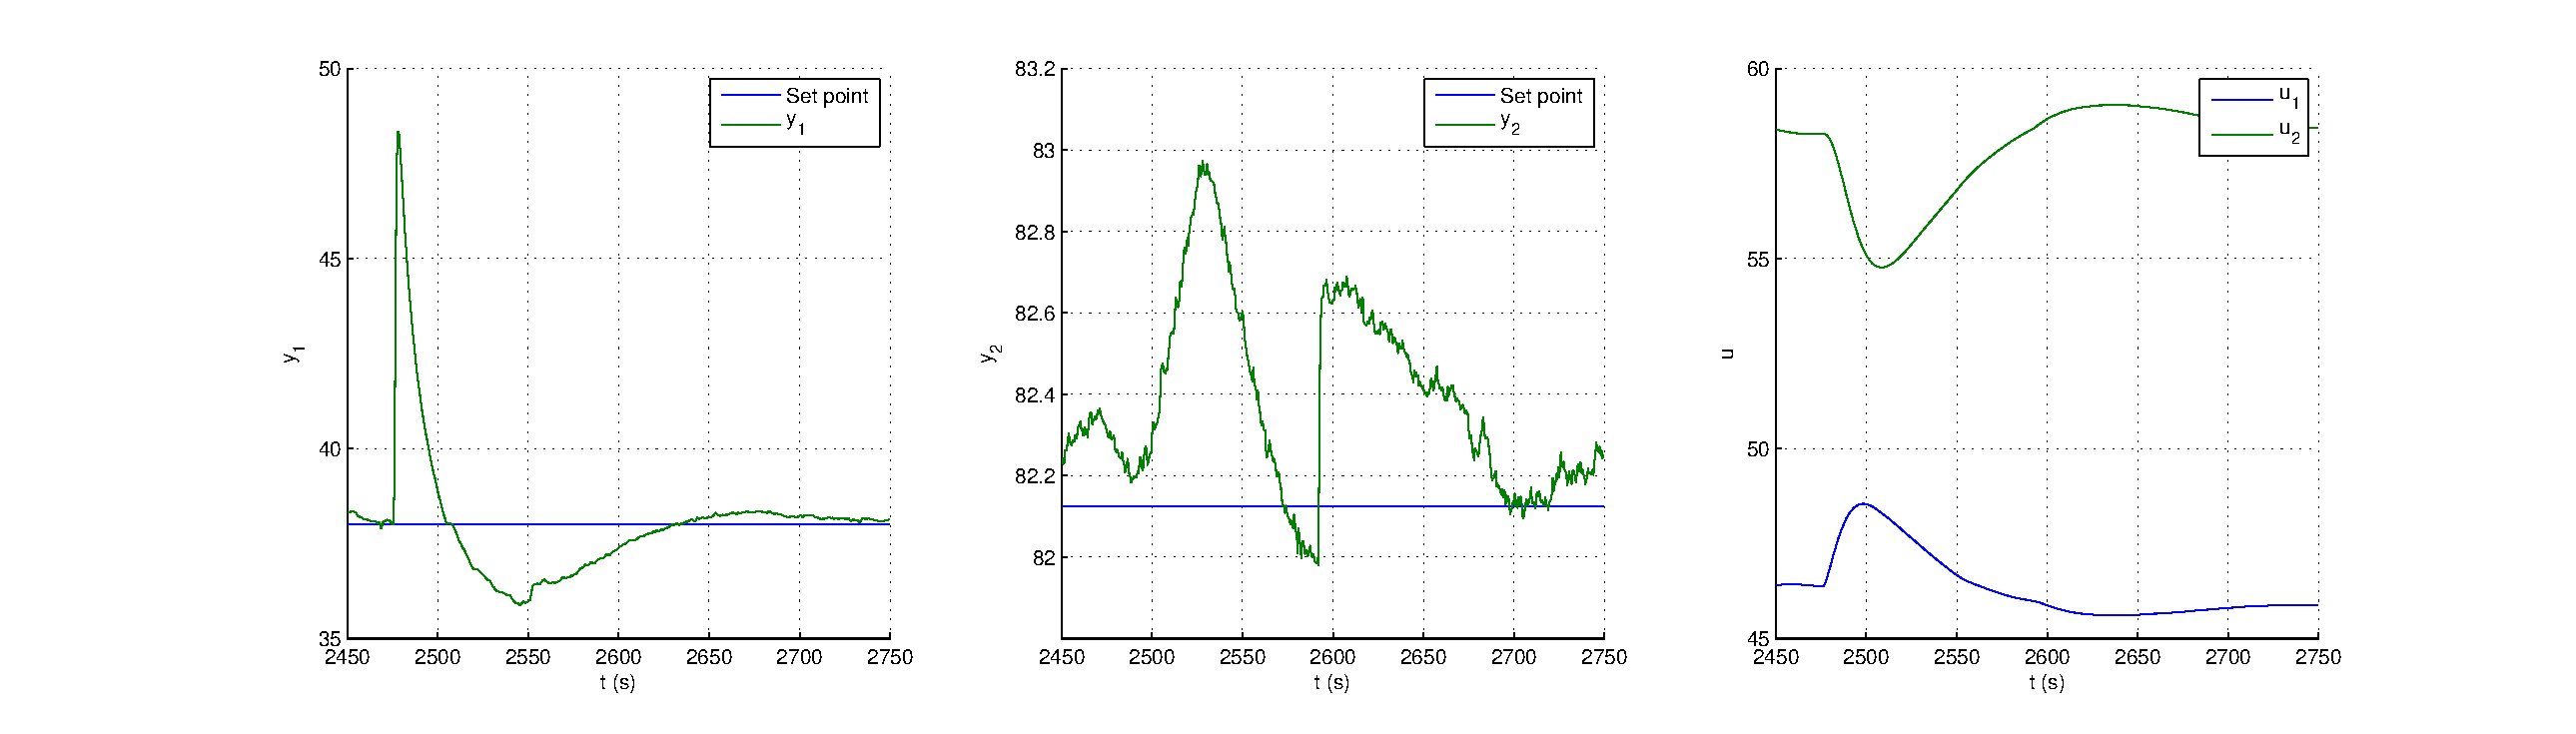
\includegraphics[width=\columnwidth]{fig/nonmin_glover_gob.eps}
                \caption{Cup of water response}
        \end{subfigure}
        \begin{subfigure}[b]{\columnwidth}
                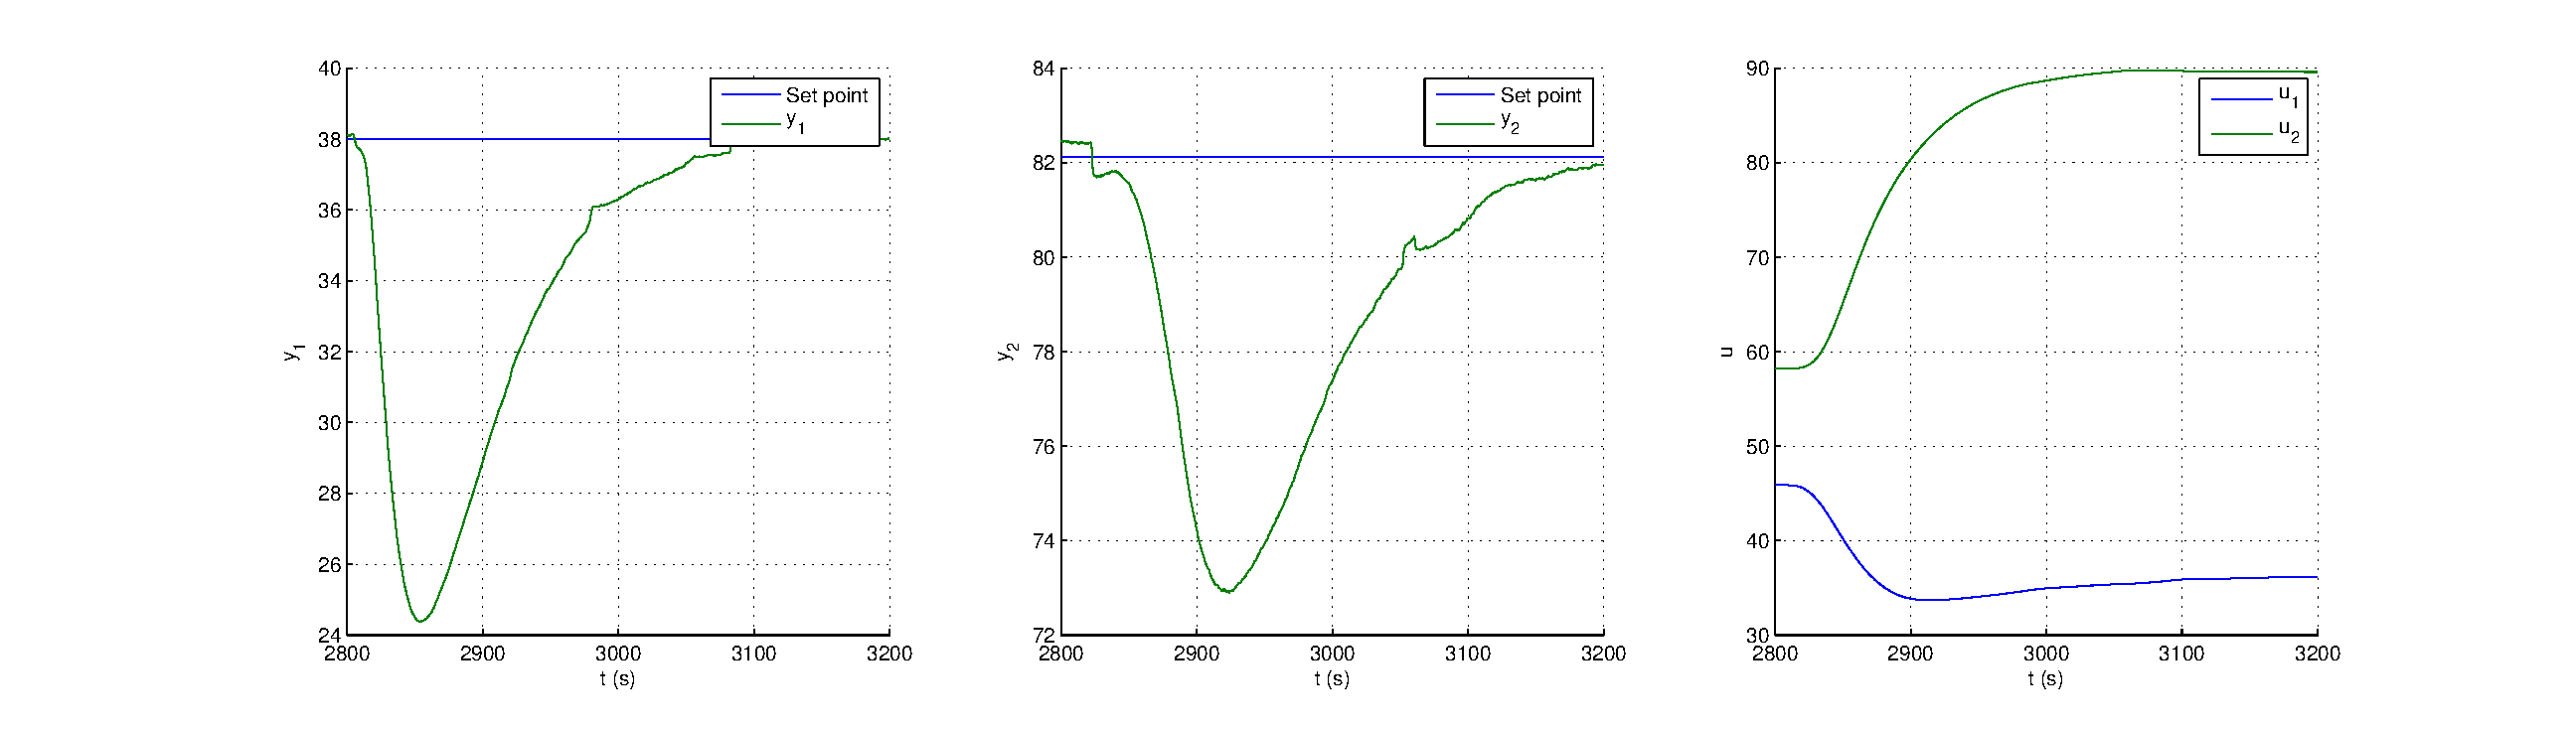
\includegraphics[width=\columnwidth]{fig/nonmin_glover_fui.eps}
                \caption{Extra outlet response}
        \end{subfigure}
        \caption{Non-minimum phase system reactions \\ Glover-MacFarlane controller}
        \label{nonmin_glover_fig}
\end{figure}

\begin{table}[h!t]
    \centering
    \begin{tabular}{|c|ccc|}
        \hline
        & Rise & \multirow{2}*{Overshoot} & Disturbance \\
        & time & & rejection \\
        Minimum phase & & & \\
        Non-minimum phase & & & \\
        \hline
    \end{tabular}
    \caption{Step response and load disturbance analysis \\ Glover-MacFarlane controllers}
    \label{analysis_glover}
\end{table}

% \subsubsection{Exercise} 

Using Glover-MacFarlane controllers lead to a huge improvement of the controlled system:
\begin{shortitemize}
    \item All time are reduced (at least by a factor 2)
    \item Overshoots are decreased (at least by a factor 5)
    \item The step responses (non-minimum case) do not go in the wrong direction
\end{shortitemize}

% \subsubsection{Exercise}\lipsum[1-1]

% \subsubsection{Exercise}

The two previous exercises lead to the design of the following controller:

$$F_r(s) = \frac{1}{1 + \tau s}$$
$$F_y(s) = K \frac{\tau_D s + 1}{\beta \tau_D s +1}\frac{s + \omega_I}{s} \frac{\omega_0^2}{(s+\omega_0)^2}G(s)^{-1} G_d(s)$$

With:

$$\begin{array}{rcl}
    \tau & = & 0.14 \text{ s}\\ 
    K &  = & 1.35\\
    \tau_D &  = & 0.078\text{ s}\\
    \beta &  = & 0.75\\
 \omega_I &  = & 5 \text{ rad.s}^{-1}\\
    \omega_0 &  = & 50 \text{ rad.s}^{-1}\\
\end{array}$$

\textbf{All the criteria are met:}

\begin{shortitemize}
    \item Rise time:
        $$t_r = 0.19\text{s}$$
    \item Overshoot:
        $$D(\%) =  2.9\%$$
    \item Step in the disturbance:
        $$|y(t)| \leq 1, \forall t \text{ and } |y(t)| \leq 0.1, \forall t \geq 0.4\text{ s}$$ 
    \item Control signal obeys:
        $$|u(t)| \leq \max_t |u(t)| = 0.98 \leq 1, \forall t$$
\end{shortitemize}

Figure \ref{designFr} shows the step response of the system, the response to a step in the disturbance and the bode diagram of the sensitivity and complementary sensitivity functions.

\begin{figure}[h!t]
    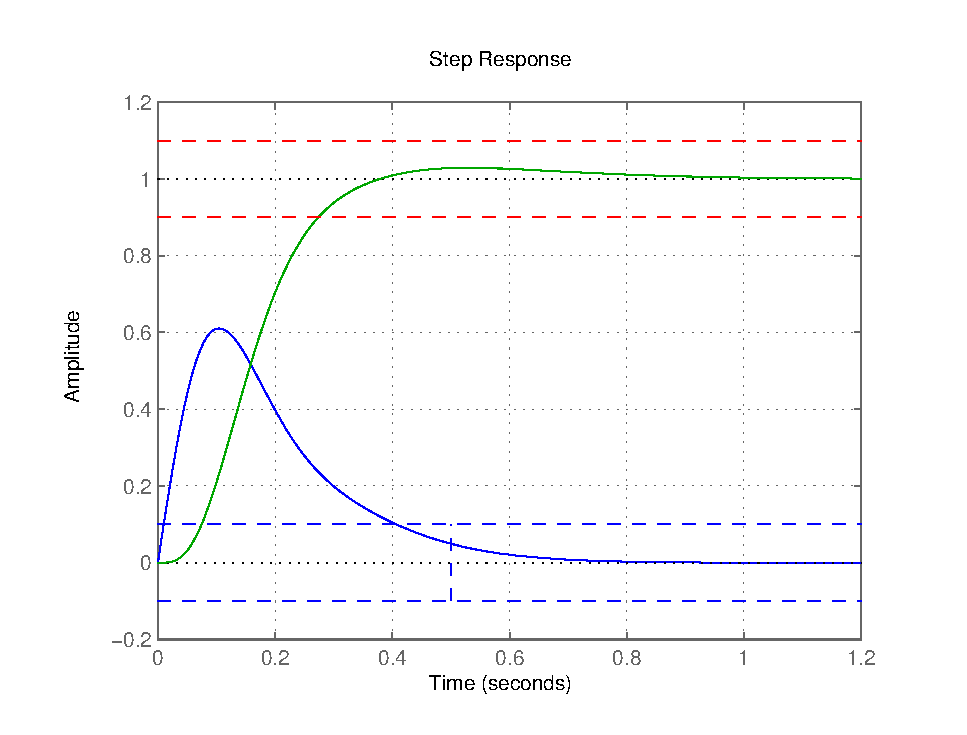
\includegraphics[width=\columnwidth]{fig/designFr.eps}
    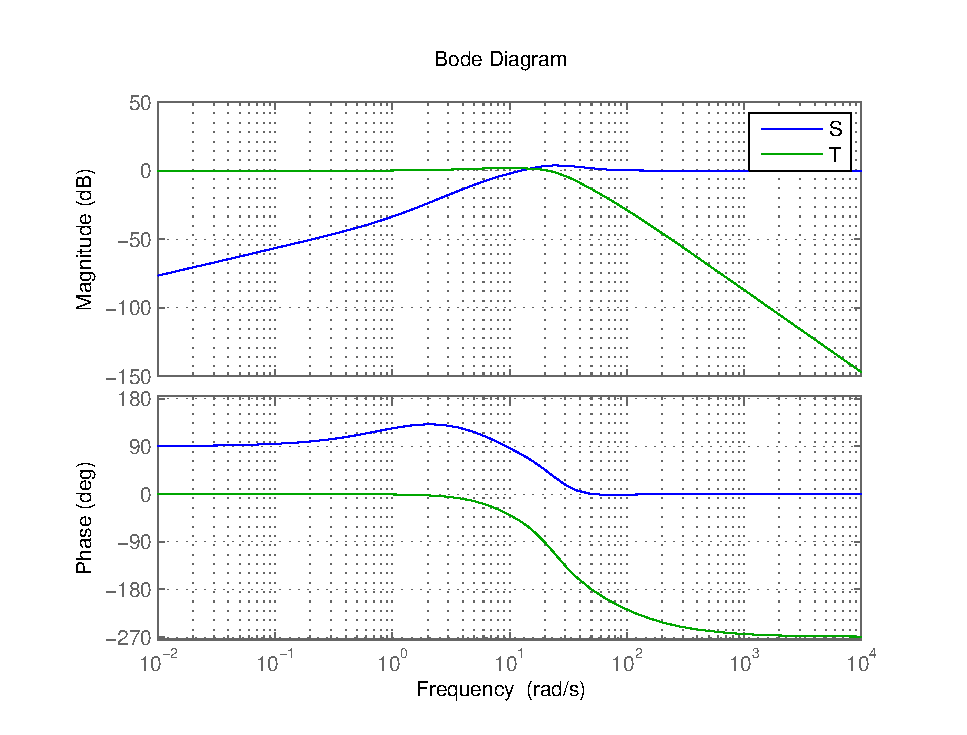
\includegraphics[width=\columnwidth]{fig/sensitivitiesFunction.eps}
    \caption{Step response of the system (green) and response to a step in the disturbance (blue) with the addition of the lead-controller \\ Bode diagram of the sensitivity and complementary sensitivity functions}
    \label{designFr}
\end{figure}



\end{document}
